%trascrizione: Costa

\titlet{Funzioni a foruncolo}

\begin{defn}[Funzione a foruncolo]
	Dati $b>a>0$, una funzione liscia
	$\fundef[\lambda] {\R^n}{\R}$
	che dipende solo da $|x|$ tale che 
	\begin{itemize}
		\item $|x|\le a\implies\lambda(x)=1$;
		\item $a<|x|<b\implies0<\lambda(x)<1$;
		\item $|x|\ge b\implies\lambda(x)=0$
	\end{itemize}
	è detta \emph{funzione a foruncolo}
	(o anche \emph{partizione dell'unità di Paley-Littlewood}).\footnotemark
	\footnotetext{In fondo alla dimostrazione del \autoref{th:ldmi}
	c'è un esempio di come costruire funzioni di questo tipo.}
	\begin{figure}
		\centering
		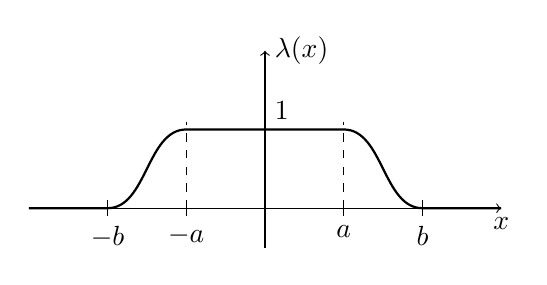
\begin{tikzpicture}
			\pgfmathsetmacro\a{1}
			\pgfmathsetmacro\b{2}
			\pgfmathsetmacro\h{(\a+\b)/2}
			\draw[->] (0,-.5) -- (0,2) node[right] {$\lambda(x)$};
			\draw[->] (-3,0) -- (3,0) node[below] {$x$};
			\foreach \x in {,-} {
				\draw (\x\a,-.1) node[below] {$\x a$} -- (\x\a,.1);
				\draw (\x\b,-.1) node[below] {$\x b$} -- (\x\b,.1);
				\draw[dashed] (\x\a,0) -- (\x\a,1.1);
				\draw[thick] (\x3,0) -- (\x\b,0) .. controls (\x\h,0) and (\x\h,1) .. (\x\a,1) -- (0,1);
			}
			\path (0,1) node[above right] {$1$};
		\end{tikzpicture}
		\caption{Funzione a foruncolo $\R\funarrow\R.$}
	\end{figure}
\end{defn}

\begin{oss}
	Nei punti in cui $\abs x = a$ tutte le derivate sono nulle, dunque $\lambda$ non è analitica.
\end{oss}

% questa cosa mi sembra senza senso, la sostituisco con supercazzola generica
% Usiamo adesso questa nozione per estendere funzioni definite localmente.
% \begin{prop}
%  Sia $M$ una varietà e $(U, \phi)$ una carta. Allora posso estenderla su tutta la varietà.
% \end{prop}
%  \begin{proof}
%   Basta considerare $\fundef[\lambda\cdot f] M\R$ con $\lambda$ a foruncolo.
%  \end{proof}

Le funzioni a foruncolo si usano per estendere
funzioni lisce $U\subseteq\R^n\funarrow\R^k$ a tutto $\R^n$:
se il dominio contiene una palla,
si moltiplica la funzione per una funzione a foruncolo
che sia nulla fuori dalla palla.
 
\titlet{Varietà con bordo}

Per definire le varietà come oggetti che localmente somigliano a $\R^n$,
abbiamo usato omeomorfismi locali con aperti di $\R^n$.
Per definire le varietà con bordo,
considereremo omeomorfismi locali con aperti di un sottoinsieme di $\R^n$ che abbia bordo.
In particolare useremo il \emph{semipiano superiore}:
\[\mathbb H^n\is[0;\infty)^n=\setdef[x\in\R^n]{\forall i:x_i\ge 0}\]

\begin{defn}[Diffeomorfismo fra sottoinsiemi arbitrari di $\R^n$]
	\label{th:arbdiffeo}
	Sia $\fundef AB$ con $A,B\subseteq \R^n$.
	$f$ è un \emph{diffeomorfismo} se
	\begin{itemize}
		\item è un omeomorfismo;
		\item
			$\forall x\in A \,\exists (U_x,\phi)$ carta locale di $\R^n$
			tale che $f|_{U\cap A}=\phi|_{U\cap A}$.
	\end{itemize}
\end{defn}

\begin{defn}[Varietà con bordo]
	$M$ è una \emph{$n$-varietà con bordo} se 
	\begin{itemize}
		\item è uno spazio topologico $T_2$ e 2-numerabile;
		\item
			è munito di atlante massimale $\set{(U_\lambda,\phi_\lambda)}$ a valori in $\mathbb H^n$,
			cioè si ha $\fundef[\phi_\lambda]{U_\lambda}{W_\lambda}$ omeomorfismo
			con $U_\lambda$ aperto di $M$ e $W_\lambda$ aperto di $\mathbb H^n$;
		\item
			$\forall \mu,\lambda:
			\phi_\mu\circ\phi_\lambda^{-1}:
			\phi_\lambda(U_\lambda\cap U_\mu) \funarrow \phi_\mu(U_\lambda\cap U_\mu)$
			è un diffeomorfismo nel senso della \autoref{th:arbdiffeo}.
	\end{itemize}
\end{defn}

\begin{defn}[Bordo]
	Il \emph{bordo} di una $n$-varietà con bordo $M$
	è costituito dai punti la cui immagine attraverso una carta
	è contenuta nella frontiera del semipiano superiore:
	\begin{gather*}
		\boundary M \is
		\setdef[x\in M]{\exists(U_x,\phi)\text{ carta locale}:\phi(x) \in \bound \mathbb H^n} \\
		\bound \mathbb H^n =
		\mathbb H^n \cap \setdef[x\in\R^n]{\exists i:x_i=0}
	\end{gather*}
	Può essere $\boundary M=\nullset$,
	nel qual caso diciamo che $M$ è senza bordo o \emph{chiusa}.
\end{defn}

\begin{ex}
	Se un punto è di bordo per una carta,
	lo è per tutte le carte che lo contengono.
\end{ex}

\begin{fat}
	Le nozioni di applicazione liscia
	e quindi di diffeomorfismo
	si estendono alle varietà con bordo.
\end{fat}

Come abbiamo fatto con le varietà differenziabili,
d'ora in poi chiameremo ``varietà'' le varietà con bordo.
Comunque,
le varietà non con bordo rientrano nel caso
di varietà con bordo chiuse.

\titlet{Sottovarietà}

\begin{defn}[Sottovarietà]
	Sia $M$ una $m$-varietà chiusa e $N\subseteq M$.
	$N$ è una \emph{sottovarietà} di dimensione $n\le m$ se
	$\forall x\in N$ esiste una carta locale $\fundef[\phi]U{W\subseteq\R^m}$
	con $\phi(U\cap N)=W\cap\R^n$,
	dove $\R^n$ è incluso in modo naturale in $\R^m$.
\end{defn}

\begin{oss}
	Una sottovarietà è una varietà.
\end{oss}

Vediamo un esempio abbastanza generale di sottovarietà:

\begin{defn}[Valore regolare]
	Sia $\fundef{U\subseteq\R^n}{\R^m}$ liscia con $U$ aperto.
 	$y\in f(U)$ è un \emph{valore regolare} per $f$ se
	$\forall x\in f^{-1}(y)$, $\de_xf$ è surgettivo.
\end{defn}

\begin{prop}
	$y$ valore regolare $\implies
	f^{-1}(y)$ sottovarietà di $U$ di dimensione $n-m$.
\end{prop}

\begin{proof}
	Segue dal \hyperref[th:funimpsurg]{teorema della funzione implicita, versione surgettiva}
	(vedi \autoref{fig:vededritto}).
	\begin{figure}
		\centering
		% questa figura era un poccio, l'ho ridisegnata
		% sono passato da psi a phi per coerenza con il teorema della funz. implicita
		% \input{diffeo.pdf_tex}
		\begin{tikzpicture}
			% cerchio a sinistra ("dritto")
			\coordinate (cc) at (-4,0);
			\draw (cc) circle (1);
			\draw[thick] (cc) +(-180:1) -- +(0:1);
			% cerchio al centro ("storto")
			\draw (0,0) circle (1.5);
			\draw[name path=N, thick] (180+10:1.5) to[bend left] (-5:1.5);
			\path[name path=vert] (90:1.5) -- (-90:1.5);
			\path[name intersections={of=N and vert, by=Nc}];
			\draw (Nc) node[above] {$f^{-1}(y)$};
			\draw (Nc) circle (1);
			% R^m a destra
			\coordinate (Rm) at (3,0);
			\path (Rm) node[right] {$\R^m$};
			% phi : cerchio dritto -> cerchio storto locale
			\path (Nc)+(180-40:1.1) coordinate (phiR);
			\draw[->, name path=phi] (cc)+(40:1.1) to[bend left] (phiR);
			\path[name path=vert2] (-2,0) +(90:2) -- +(-90:2);
			\path[name intersections={of=phi and vert2, by=phic}];
			\path (phic) node[above] {$\phi$};
			% f : cerchio storto -> R^m
			\path (Rm)+(0,.2) coordinate (Rma);
			\draw[->, name path=f] (20:1.6) to[bend left] (Rma);
			\path[name path=vert3] (2.3,0) +(90:2) -- +(-90:2);
			\path[name intersections={of=f and vert3, by=fc}];
			\path (fc) node[above] {$f$};
			% pi : cerchio dritto -> R^m
			\path (Rm)+(0,-.2) coordinate (RmS);
			\draw[->, name path=pi] (cc)+(-40:1.1) to[out=-40, in=180+50] (RmS);
			\path[name path=vert4] (cc)++(1.5,0) +(90:2) -- +(-90:2);
			\path[name intersections={of=pi and vert4, by=pic}];
			\path (pic) node[above right] {$\pi$};
		\end{tikzpicture}
		\caption{$\phi^{-1}$ è una carta locale per $f^{-1}(y)$ (``vede dritto'').}
		\label{fig:vededritto}
	\end{figure}
\end{proof}

Usando l'ultima proposizione otteniamo
$S^n$ come sottovarietà di $\R^{n+1}$:
\[S^n=r^{-1}(1),\quad
r(x)\is\sqrt{x_1^2+\dots+x_{n+1}^2}\]

Segue un risultato analogo con il differenziale iniettivo:

\begin{prop}
	Se $\forall x \in U:\de_xf$ è iniettiva
	e $\fundef U{f(U)}$ è un omeomorfismo,
	allora $f(U)$ è una sottovarietà di $\R^m$
	con $f$ diffeomorfismo.
\end{prop}

\begin{proof}
	Segue dal \hyperref[th:funimpinj]{teorema della funzione implicita, versione iniettiva}.
\end{proof}

\begin{oss}
	Nel teorema sopra l'ipotesi di omeomorfismo è necessaria!
	Come controesempio basta prendere:
	\begin{center}
		\input{trifoglio.pdf_tex}
	\end{center}
	Nel cerchio tratteggiato si ha il problema: ci sono 3 ``rami''!
\end{oss}

\paragraph{Bordo}

Nel caso di varietà non chiuse
abbiamo tre modelli locali possibili
al variare del domicilio di una $n$-sottovarietà contenuta in una $m$-varietà:
\begin{enumerate}
 \item il bordo di $\mathbb H^n$ non sta nel bordo di $\mathbb H^m$;
 \item il bordo sta nel bordo;
	 \label{it:svpropria}
 \item caso misto.
\end{enumerate}
\begin{center}
	\input{modellobordo.pdf_tex}
\end{center}

\begin{defn}[Sottovarietà propria]
	$N\subseteq M$ è \emph{sottovarietà propria}
	se l'unico modello che si realizza è (\ref{it:svpropria}),
	ossia $\boundary N = N\cap \boundary M$.
\end{defn}
